% Preprint: conjunctival pallor screening on CP-AnemiC
% Build: tectonic main.tex
% Figures are read from ../results/, regenerated by scripts/run_full_analysis.py
%         and scripts/make_extra_figures.py
\documentclass[11pt,a4paper]{article}

\usepackage[margin=2.5cm]{geometry}
\usepackage[T1]{fontenc}
\usepackage{lmodern}
\usepackage{microtype}
\usepackage{amsmath,amssymb}
\usepackage{booktabs}
\usepackage{graphicx}
\usepackage{caption}
\usepackage{siunitx}
\usepackage[hidelinks]{hyperref}
\usepackage{xcolor}
\usepackage{authblk}
\usepackage{abstract}

\captionsetup{font=small,labelfont=bf}
\sisetup{detect-weight=true}

\newcommand{\gdl}{\ensuremath{\mathrm{g/dL}}}
\newcommand{\auroc}{AUROC}

\title{\bfseries Duplicate leakage in a public conjunctival pallor benchmark,\\
and an honest baseline for image-based anaemia screening}

\author[1]{Paing Hein Htet}
\affil[1]{Department of Medical Physics and Biomedical Engineering,
University College London, London, United Kingdom}
\affil[ ]{\texttt{zcemphh@ucl.ac.uk}}
\date{\today}

\begin{document}
\maketitle

\begin{abstract}
\noindent
Conjunctival pallor photographs are an attractive substrate for non-invasive anaemia
screening, and CP-AnemiC --- 710 images of Ghanaian children aged 6--59 months with paired
laboratory haemoglobin --- has become a convenient public benchmark for the task. We report
that the benchmark contains duplication substantial enough to change published
conclusions, and we provide a corrected baseline.

Only 383 of the 710 metadata rows are distinct photographs. The duplication takes three forms,
each of which defeats the detection method that sufficed for the previous one: 212 byte-identical copies; 19 re-encoded copies whose
bytes, and so whose hashes, differ; and 96 \emph{shifted or re-cropped} copies whose hand-drawn
masks differ as well, so that neither hashing nor bounding-box pixel comparison detects them.
116 groups carry \emph{conflicting} haemoglobin labels on the same photograph, one spanning 3.3
to 10.4~\gdl. Because copies are frequently attributed to different hospitals, the redundancy
defeats site-grouped cross-validation as well as random splits: under hash and aligned-pixel
deduplication with site-grouped folds, 74 photographs still enter the analysis as 164 rows across
different site folds. A random split inflates \auroc{} by $+0.176$ (95\,\% CI $+0.120$ to
$+0.232$, $n_{\text{boot}}=5000$); a matched-$n$ control attributes about half of the final
deduplication step to leakage and about half to the smaller resulting sample.

After removing all three forms and grouping by collection site, twelve interpretable colour
features reach \auroc{} $0.706$ (95\,\% CI $0.653$--$0.757$) for WHO anaemia
($\mathrm{Hb}<11$~\gdl), against a demographics-only floor of $0.524$; the image contributes
$+0.182$ \auroc{} (DeLong 95\,\% CI $+0.107$ to $+0.258$, $p=2.1\times10^{-6}$). Bland--Altman
limits of agreement span $7.8$~\gdl{} with strong proportional bias (slope $-0.81$), so the model
is a triage screen and not a haemoglobin meter. At 90\,\% sensitivity, specificity falls to
$0.303$, and decision curve analysis places the model below referring every child up to a threshold
probability of about $0.26$ --- it is useful only where confirmatory testing is scarce.

We recommend that future work on CP-AnemiC deduplicate under small translations, not merely by file
hash or aligned pixel comparison, and we release the detector and full analysis so that reported
numbers can be checked against these controls.
\end{abstract}

\medskip
\noindent\textbf{Keywords:} anaemia screening; conjunctival pallor; data leakage;
benchmark integrity; medical imaging; low-resource diagnostics.

\section{Introduction}

Anaemia affects an estimated 40\,\% of children aged 6--59 months worldwide, rising to
68\,\% in west and central Africa~\cite{stevens2022}, and diagnosis
conventionally requires a blood draw and laboratory or point-of-care haemoglobin assay.
Both are constrained in low-resource settings by cost, consumables, trained staff and
infection-control requirements. This has motivated interest in image-based screening: the
palpebral conjunctiva is a mucous membrane whose colour is visibly influenced by
haemoglobin concentration, is straightforward to expose, and can be photographed with a
consumer smartphone.

Public datasets are what allow such methods to be compared. CP-AnemiC
\cite{asare2023cpanemic} pairs conjunctiva photographs of Ghanaian children with laboratory
haemoglobin and has been adopted as a benchmark for this task. The value of any benchmark,
however, rests on an assumption that is rarely re-examined once a dataset is in circulation:
that its records are distinct. Where they are not, a randomly partitioned evaluation places
copies of the same photograph in both training and test folds, and the resulting score
measures memorisation rather than generalisation.

This paper makes three contributions.

\begin{enumerate}
  \item We show that CP-AnemiC contains duplicate records in three forms --- byte-identical,
        re-encoded, and shifted or re-cropped --- at a scale that materially inflates reported
        performance, and we quantify that inflation. The third form is detectable only under
        translation alignment, and because its members are frequently attributed to different
        hospitals it defeats site-grouped validation as well as random splits.
  \item We establish a corrected baseline under full deduplication and site-grouped
        cross-validation, using interpretable colour features only.
  \item We characterise the resulting model as a screening instrument --- reporting the
        operating point, calibration and Bland--Altman agreement that determine whether it
        could be deployed --- and conclude that it is not yet adequate as a haemoglobin
        estimator.
\end{enumerate}

We propose no new architecture; the aim is to establish what this benchmark supports under
stated controls, and to make those controls reproducible.

\section{Data}

\subsection{Source}

CP-AnemiC \cite{asare2023cpanemic} comprises conjunctiva photographs of children aged
6--59 months collected at ten hospitals across four Ghanaian regions, each paired with a
laboratory haemoglobin measurement. Ages in the distributed spreadsheet are bucketed (11, 12, 24,
36, 48 and 60 months), and 90 rows are coded at 60 months, marginally outside the stated band; we
use age only as a demographic covariate and as the demographics-only baseline. We use the WHO threshold for childhood anaemia,
$\mathrm{Hb}<11$~\gdl~\cite{who2011}. Table~\ref{tab:data} summarises the dataset as distributed and after
the deduplication described below.

\begin{table}[htbp]
\centering
\caption{CP-AnemiC as distributed and after deduplication.}
\label{tab:data}
\small
\begin{tabular}{lr}
\toprule
Property & Value \\
\midrule
Metadata rows (as distributed)          & 710 \\
Distinct files by SHA-256 (pass 1)      & 498 \\
Distinct after re-encode merge (pass 2) & 479 \\
\textbf{Distinct photographs after alignment (pass 3)} & \textbf{383} \\
Rows whose file hash appears exactly once & 407 \\
Duplicate groups with conflicting Hb (hash grain) & 90 \\
\quad the same, at the 383-photograph grain & 116 \\
Groups attributed to more than one hospital & 125 \\
Collection sites                    & 10 hospitals, 4 regions \\
Cohort                              & children 6--59 months \\
Label                               & laboratory Hb (\gdl); WHO threshold 11 \\
Anaemia prevalence after dedup      & 0.509 \\
\bottomrule
\end{tabular}
\end{table}

\subsection{Duplicate structure}

Three distinct forms of redundancy are present, and each is invisible to the method that
suffices for the one before it.

\emph{Byte-identical} duplication accounts for 212 files: the same image registered under more
than one identifier, detectable by hashing the file (710 $\to$ 498).

\emph{Re-encoded} copies account for a further 19: the same photograph written to disk again,
so the bytes and therefore the hash differ. Thirteen are exactly pixel-identical once the
region of interest is extracted and six differ only by a small crop or in under 2\,\% of
pixels. Detecting them requires comparing decoded pixels within the annotated region
(498 $\to$ 479).

\emph{Shifted or re-cropped} copies are the largest group, at 96, and the least visible. Here
the photograph is the same but the hand-drawn mask is not, so the region of interest is
translated or trimmed relative to its twin. Both the file hash and the bounding-box-normalised
pixel comparison fail: the bytes differ, and the extracted regions no longer align. Detecting
them requires searching over small translations at full resolution (479 $\to$ 383).
Figure~\ref{fig:dupes} shows one such pair.

The consequential subsets are two. At the final grain, 116 groups carry conflicting haemoglobin
labels on the same photograph --- one spanning 3.3 to 10.4~\gdl. Because the pixels are the
same, no model can satisfy both labels; the disagreement is irreducible label noise that places
a ceiling on achievable performance. Where duplicates were merged we took the median
haemoglobin, which is a defensible summary but cannot recover the truth. Separately, 125 groups
are attributed to more than one hospital, and this is the more damaging property for evaluation.
Grouping folds by collection site --- the standard remedy for site-specific confounds --- cannot
keep copies together when the copies disagree about which site they came from. Concretely, under a
protocol that deduplicates by hash and by aligned pixels and then groups by site, 74 photographs
still enter the analysis as 164 separate rows assigned to more than one site fold; under hash-only
deduplication, 83 do. A protocol we would previously have called correct still leaks.

\begin{figure}[htbp]
\centering
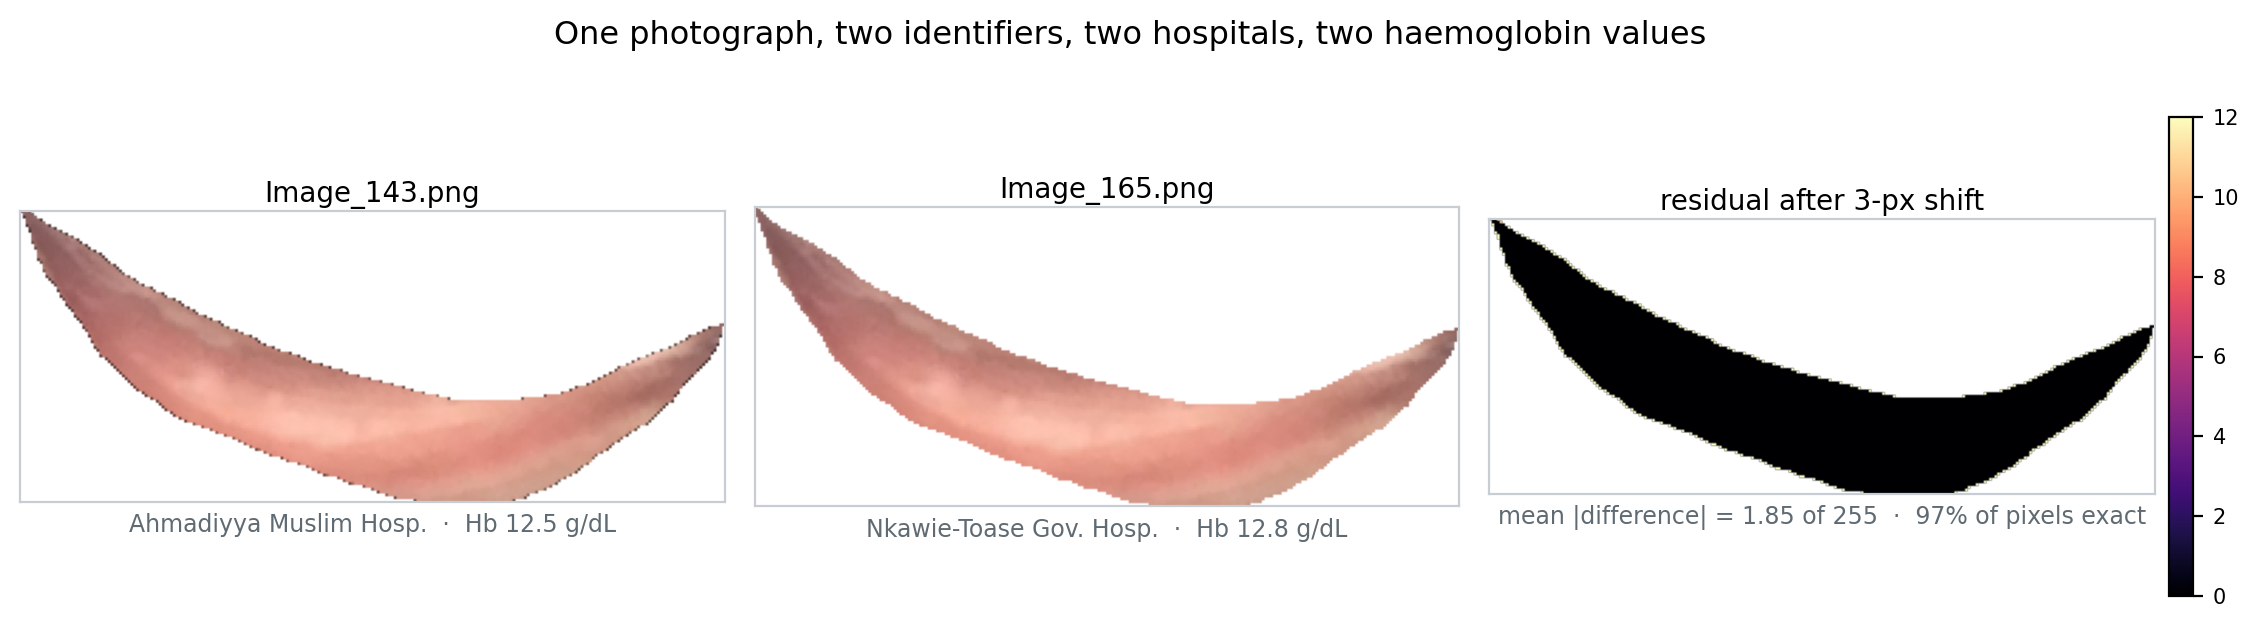
\includegraphics[width=\textwidth]{../results/fig13_shifted_pair.png}
\caption{A shifted duplicate pair. The two files have different SHA-256 hashes, different
hand-drawn masks, and are attributed to different hospitals with different haemoglobin values.
After a three-pixel vertical shift, 97\,\% of overlapping pixels are exactly equal and the mean
absolute difference is $1.85$ of $255$ --- a residual consistent with re-compression, not with
two photographs. Neither file hashing nor bounding-box pixel comparison detects this pair.}
\label{fig:dupes}
\end{figure}

\subsection{Mask handling}

Each image is RGBA, where the alpha channel is a hand-drawn conjunctiva mask covering
approximately 25\,\% of the frame; the remainder is black padding. Colour statistics must
therefore be computed over masked pixels only. Ignoring the mask shifts mean RGB by more
than $100/255$ and produces features that encode \emph{mask area} --- an artefact of
annotator behaviour --- rather than tissue colour.

\section{Methods}

\subsection{Features}

We extract twelve interpretable colour features over the masked region of interest: mean
$R$, $G$, $B$; circular mean hue and hue concentration; mean saturation; CIELAB $L^*$,
$a^*$, $b^*$; an illumination-normalised redness index $r/(r+g+b)$; its 10th percentile; and
the red/green ratio. The $a^*$ channel is the perceptual red--green axis that corresponds to
what a clinician reads as pallor.

Two exclusions are deliberate. \textbf{Mask area is not used as a feature}: it reflects how
the annotator drew the boundary rather than physiology, and had it correlated with site or
severity the model would have learned the annotator. \textbf{Hue is averaged circularly}:
red tissue sits near both $0.0$ and $1.0$ on the hue circle, so a linear mean of $0.98$ and
$0.02$ returns $0.5$, which is cyan.

\subsection{Model and validation}

A gradient-boosted regressor predicts haemoglobin; negating its output yields a screening
score. Hyperparameters were fixed \emph{a priori} and never tuned on this data; a nested
cross-validation check (Section~\ref{sec:controls}) confirms they were not selected for
flattery: tuning inside each fold scores lower, not higher.
All reported metrics are out-of-fold.

\paragraph{Deduplication.} Three passes run in sequence, each addressing what the previous one
cannot see. Pass 1 hashes file bytes with SHA-256. Pass 2 decodes each remaining image, crops to
the conjunctiva mask's bounding box, downsamples to $32\times32$ and merges pairs whose mean
absolute difference falls below 3.0 on the 0--255 scale; merged pairs all lie below $2.1$ while
the closest distinct pair sits at $4.1$, so the threshold occupies a measured gap. Pass 3 targets
copies whose masks differ, which defeats the bounding-box normalisation of pass 2: candidate pairs
--- taken from the union of a generous thumbnail cut-off and a translation-invariant colour
histogram, so that a mask mismatch cannot hide a pair from both --- are verified at full
resolution by the smallest masked mean absolute difference over integer translations up to
$\pm30$~px. Same-capture pairs sit below $2.7$; visually distinct repeat captures begin at $3.1$,
and we place the threshold at 3.0 within that gap after inspecting the borderline pairs by eye.
All merges use union--find, so a chain of copies collapses to one photograph.

\paragraph{Cross-validation.} Folds are grouped by collection site, so that a model cannot exploit
site-specific camera, lighting or operator signatures shared between training and test folds. We
report a waterfall over both requirements. Neither requirement alone is
sufficient here. After hashing and the re-encode merge, 74 photographs still appear as multiple
rows attributed to different hospitals, so site-grouping cannot contain them; and because those
rows differ in bytes and in mask, hashing and bounding-box comparison do not remove them either.
Where a merged group spans several sites we assign it the site of its first-listed member, a
convention rather than a fact: 125 of the 383 groups have no unambiguous site.

\section{Results}

\subsection{Progressive removal of optimism}

Table~\ref{tab:waterfall} evaluates the same colour features under successively stricter
protocols. Each row closes one more leak than the row above.

\begin{table}[htbp]
\centering
\caption{Effect of evaluation protocol on apparent performance. Colour features only.}
\label{tab:waterfall}
\small
\begin{tabular}{lrcc}
\toprule
Configuration & $n$ & \auroc{} [95\,\% CI] & MAE (\gdl) \\
\midrule
Random split, duplicates kept \emph{(common)} & 710 & 0.883 [0.858--0.906] & 1.46 \\
Byte-identical removed, random split                & 498 & 0.796 [0.758--0.834] & 1.44 \\
\quad + grouped by collection site                  & 498 & 0.809 [0.772--0.847] & 1.42 \\
\quad + re-encoded copies removed                   & 479 & 0.780 [0.737--0.818] & 1.46 \\
\textbf{\quad + shifted/re-cropped copies removed (headline)}
                                                    & \textbf{383}
                                                    & \textbf{0.706 [0.653--0.757]}
                                                    & \textbf{1.60} \\
\bottomrule
\end{tabular}
\end{table}

The naive configuration --- a random split with duplicates retained, which is the default when a
dataset is assumed clean --- reports \auroc{} $0.883$. The corrected protocol reports $0.706$. A
bootstrap over 5000 resamples places the total inflation at $+0.176$ (95\,\% CI $+0.120$ to
$+0.232$; the interval excludes zero). That interval and the DeLong intervals in
Table~\ref{tab:ablation} are computed on overlapping data and are not independent tests.
Figure~\ref{fig:leakage} shows the waterfall.

The final step merits separate attention. Removing shifted and re-cropped copies costs a further
$0.073$ \auroc{}. That step does two things at once, however --- it removes leakage \emph{and} it
removes 96 rows --- so the drop must be decomposed before it is credited to leakage. Subsampling
the 479-photograph set down to 383 rows at random, leaving its leakage intact, gives
$0.744 \pm 0.021$ over 25 draws. Roughly half of the $0.073$ is therefore attributable to the
smaller sample ($0.036$) and roughly half to the leakage the pass removes ($0.038$). We report
both, because a step that deletes data will always depress a learning-curve-limited estimate, and
attributing the whole of it to leakage would overstate the case.

An analysis that hashed files and grouped folds by site would stop at $0.780$.

\begin{figure}[htbp]
\centering
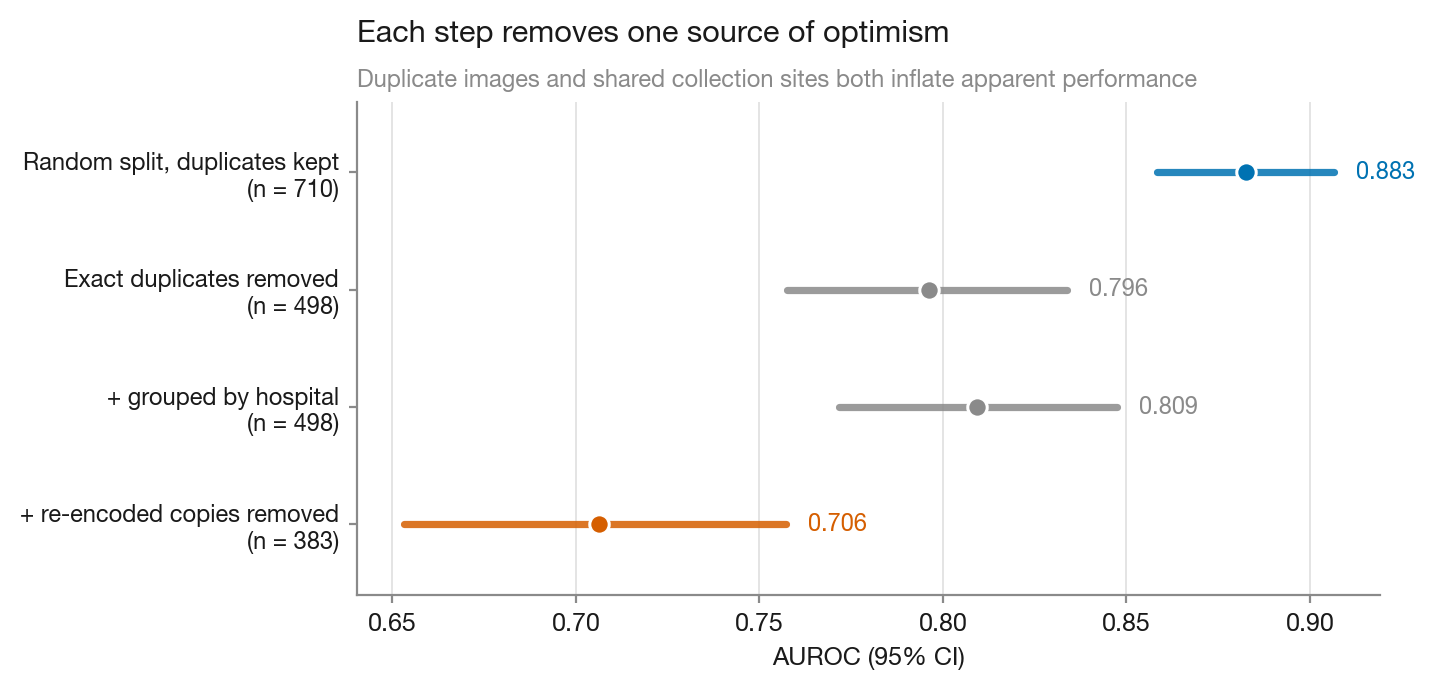
\includegraphics[width=0.78\textwidth]{../results/fig2_leakage.png}
\caption{Apparent performance under successively stricter protocols. The fall is not uniform:
removing byte-identical duplicates costs $0.087$, grouping by hospital then \emph{raises} the
estimate by $0.013$ (site grouping removes a confound but also changes the fold composition), and
the two content-based passes cost $0.029$ and $0.073$. The gap between the first and last bars is
the optimism introduced by evaluating on a benchmark whose records are not distinct.}
\label{fig:leakage}
\end{figure}

\subsection{Does the image contribute?}

A screening score could in principle be driven by demographics alone. Table~\ref{tab:ablation}
rules this out.

\begin{table}[htbp]
\centering
\caption{Feature ablation under the corrected protocol ($n=383$). Comparisons by DeLong's test~\cite{delong1988}.}
\label{tab:ablation}
\small
\begin{tabular}{lcc}
\toprule
Feature set & \auroc{} [95\,\% CI] & vs.\ colour \\
\midrule
Demographics only (age, sex) & 0.524 [0.468--0.582]
  & $\Delta = -0.182$, $p=2.1\times10^{-6}$ \\
\textbf{Colour only}         & \textbf{0.706 [0.653--0.757]} & --- \\
Colour + demographics        & 0.699 [0.647--0.751]
  & $\Delta = -0.008$, $p=0.55$ \\
\bottomrule
\end{tabular}
\end{table}

The image carries substantial and highly significant signal over demographics, and the
demographics-only floor is now close to chance ($0.524$, CI spanning $0.5$) --- the earlier,
higher floor was itself partly a duplicate artefact. Adding demographics to colour produces no
detectable improvement, the expected result if the photograph already encodes what age and sex
would otherwise proxy. The central claim of the paper survives the full deduplication: whatever
else the third pass removed, it did not remove the image signal.
Figure~\ref{fig:roc} shows the corresponding ROC curves.

\begin{figure}[htbp]
\centering
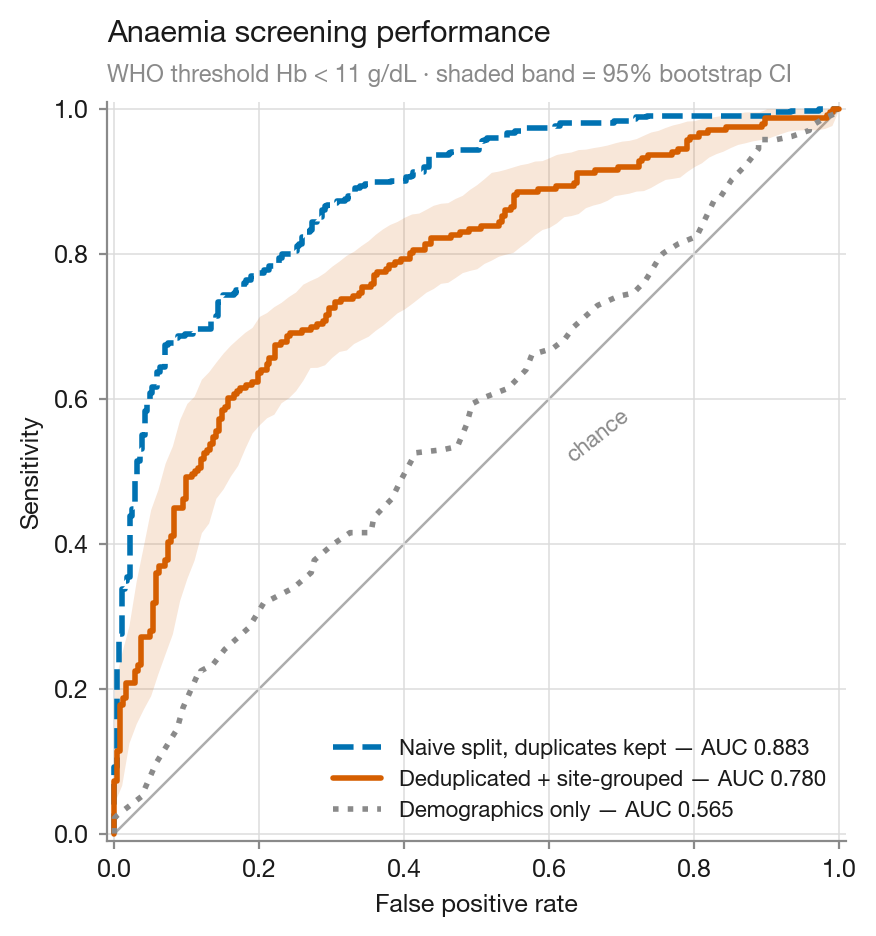
\includegraphics[width=0.68\textwidth]{../results/fig1_roc.png}
\caption{ROC curves. The corrected protocol ($0.706$) sits well below the naive leaky split
($0.883$) and well above the demographics-only floor ($0.524$). The colour + demographics variant
is omitted from the plot; it is indistinguishable from colour alone (Table~\ref{tab:ablation}).}
\label{fig:roc}
\end{figure}

\subsection{Choice of model}

We report both a haemoglobin regressor and a direct binary classifier
(Table~\ref{tab:models}), because they answer different questions and we did not wish to adopt the
better number after the fact.

\begin{table}[htbp]
\centering
\caption{Regressor versus direct classifier.}
\label{tab:models}
\small
\begin{tabular}{lccc}
\toprule
Model & \auroc{} [95\,\% CI] & Hb output & Agreement assessable \\
\midrule
Hb regressor \emph{(headline)} & 0.706 [0.653--0.757] & yes, MAE 1.60~\gdl & yes \\
Binary classifier              & \textbf{0.733 [0.680--0.785]} & no & no \\
\bottomrule
\end{tabular}
\end{table}

The classifier discriminates better, as expected when the decision is optimised directly,
but it produces no haemoglobin estimate and therefore cannot be examined for clinical
agreement. We retain the regressor as the headline because the agreement result
(Section~\ref{sec:agreement}) is the more consequential finding.

\subsection{Calibration}

\begin{table}[htbp]
\centering
\caption{Post-hoc calibration improves calibration at a cost in discrimination. Isotonic
calibration applied via \texttt{CalibratedClassifierCV} with $cv=3$.}
\label{tab:calib}
\footnotesize
\begin{tabular}{lccccc}
\toprule
Variant & Brier & ECE & H--L $p$ & \auroc{} & prob.\ range \\
\midrule
\textbf{Uncalibrated} & 0.220 & 0.114 & $<0.001$ & \textbf{0.733} & [0.01, 0.98] \\
Isotonic & 0.220 & \textbf{0.079} & \textbf{0.156} & 0.711 & [0.10, 0.84] \\
\bottomrule
\end{tabular}
\end{table}

Neither variant yields probabilities fit to report. The uncalibrated model discriminates better
but is clearly miscalibrated (Hosmer--Lemeshow $p<0.001$, ECE $0.114$); isotonic calibration
repairs the calibration --- Hosmer--Lemeshow rises to $0.156$ and ECE falls to $0.079$ --- while
costing $0.022$ \auroc{} and compressing the probability range to $[0.10, 0.84]$. The
compression is the mechanism: \texttt{CalibratedClassifierCV} fits $k$ sub-models on $k-1$ folds
each and averages them, and at roughly 300 training rows per fold each sub-model is data-starved,
so averaging pulls estimates toward the centre.

We report the uncalibrated model as the headline because the instrument is a ranking triage
screen, for which discrimination is the operative property, and we make the trade explicit rather
than choosing the flattering column. This model can order children by risk, but its output should not be read as a probability of
anaemia. We note that
this section previously reported the opposite conclusion --- that calibration degraded both
properties --- on the incompletely deduplicated data; the reversal is a reminder that
model-selection findings inherit whatever contamination the evaluation set carries.

\begin{figure}[htbp]
\centering
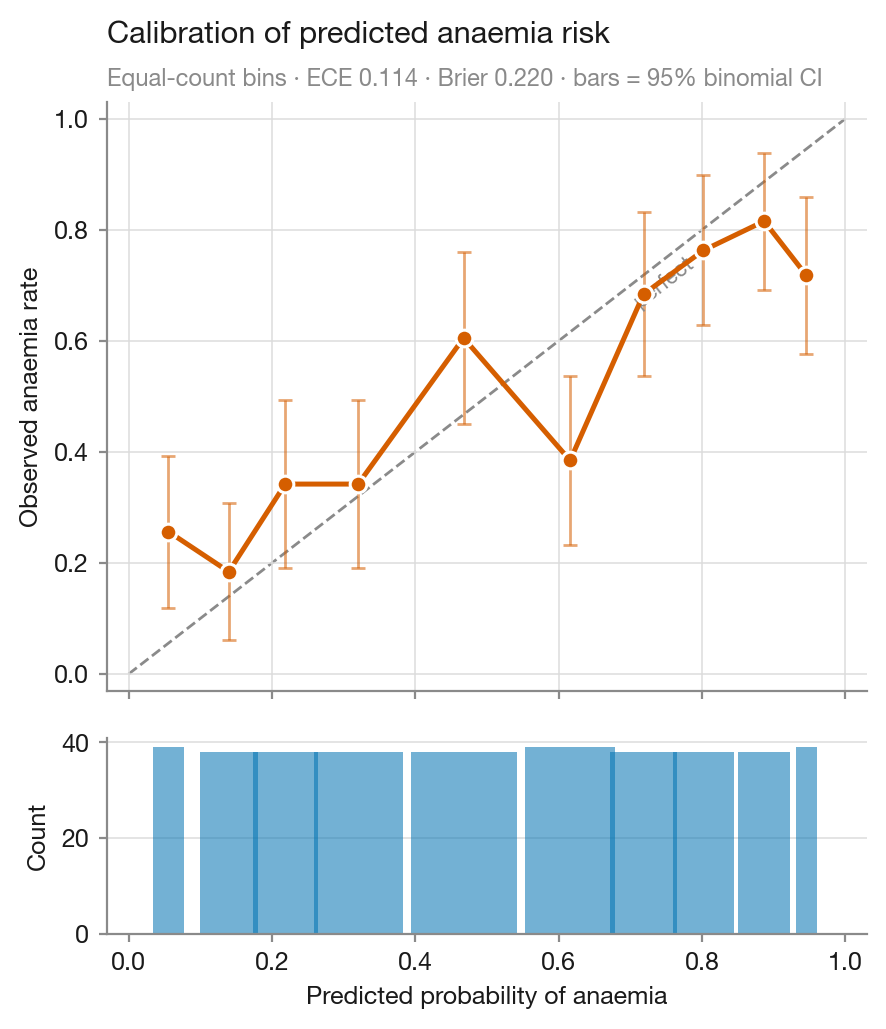
\includegraphics[width=0.68\textwidth]{../results/fig4_calibration.png}
\caption{Reliability curve for the uncalibrated model, with equal-count bins and binomial
intervals. The isotonic variant is not plotted; its summary statistics are in
Table~\ref{tab:calib}.}
\label{fig:calib}
\end{figure}

\subsection{Screening operating point}

At the WHO threshold the model achieves sensitivity $0.713$ and specificity $0.532$
(Figure~\ref{fig:op}). Tuned to
catch 90\,\% of anaemic children, specificity falls to $0.303$ --- referring roughly 70\,\% of
healthy children for confirmatory testing. At this cohort's prevalence that is about 80 referrals
per 100 children screened, against 100 for referring everyone: the screen saves roughly a fifth of
confirmatory tests while missing one anaemic child in ten. This, rather than \auroc{}, is the
quantity that determines deployability, and at present it is not good enough for unsupervised
use.

\begin{figure}[htbp]
\centering
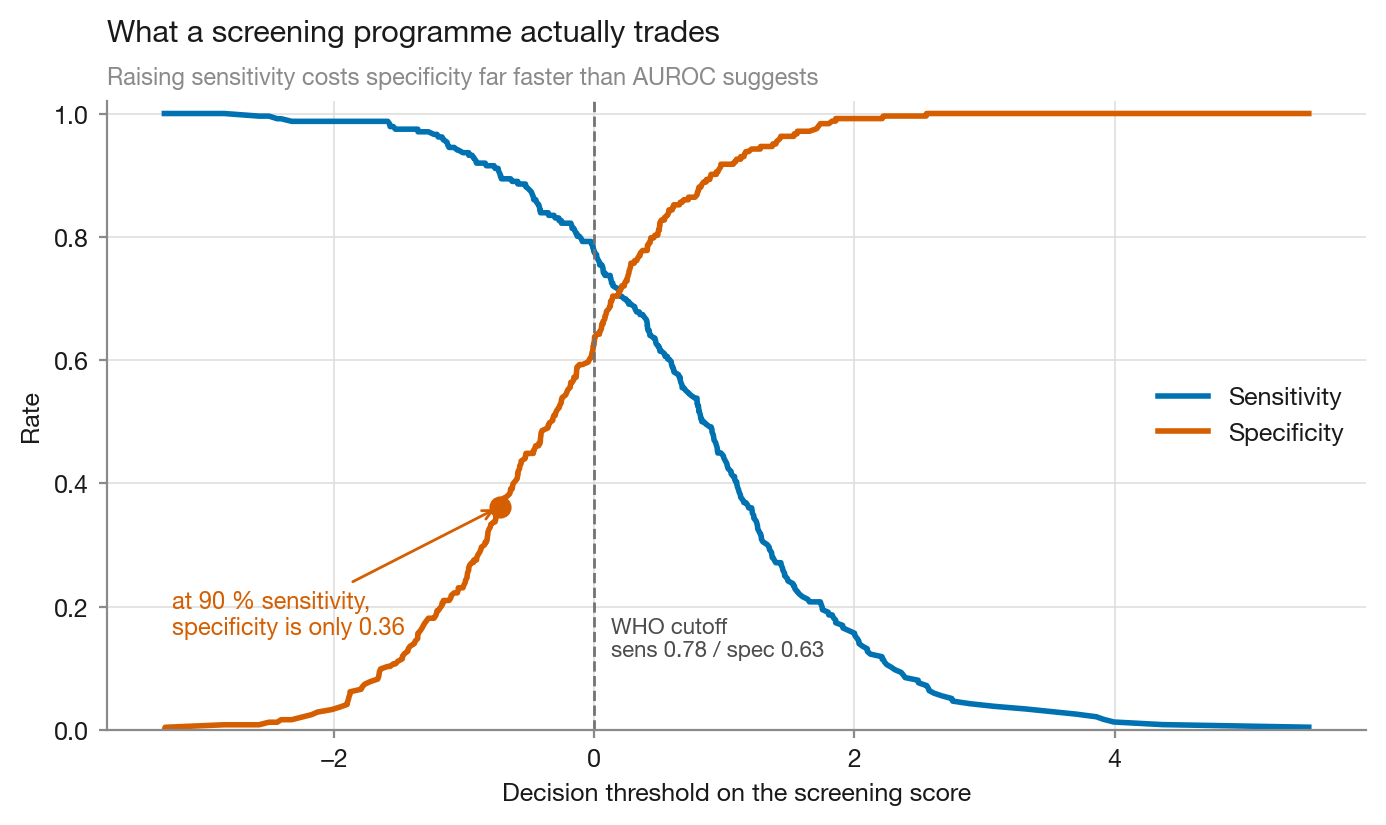
\includegraphics[width=0.82\textwidth]{../results/fig9_operating_point.png}
\caption{Sensitivity and specificity against the decision threshold, from the same out-of-fold
predictions as the headline result. The curves cross steeply: moving from the WHO cutoff to
90\,\% sensitivity costs roughly half the specificity. This trade, rather than \auroc{}, is what a
screening programme has to absorb.}
\label{fig:op}
\end{figure}

\subsection{Agreement as a haemoglobin estimator}
\label{sec:agreement}

Bland--Altman analysis~\cite{blandaltman1986} gives a bias of $+0.03$~\gdl{} with limits of agreement from $-3.87$
to $+3.92$~\gdl, a span of $7.8$~\gdl, and a proportional-bias slope of $-0.81$. The model
shrinks toward the population mean (Figure~\ref{fig:pva}), over-predicting in anaemic children
and under-predicting in healthy ones; Figure~\ref{fig:ba} shows the agreement plot itself. A clinically useful non-invasive haemoglobin meter would require limits
nearer $\pm1$~\gdl. \textbf{No haemoglobin value from this model should be reported to a
clinician.}

\begin{figure}[htbp]
\centering
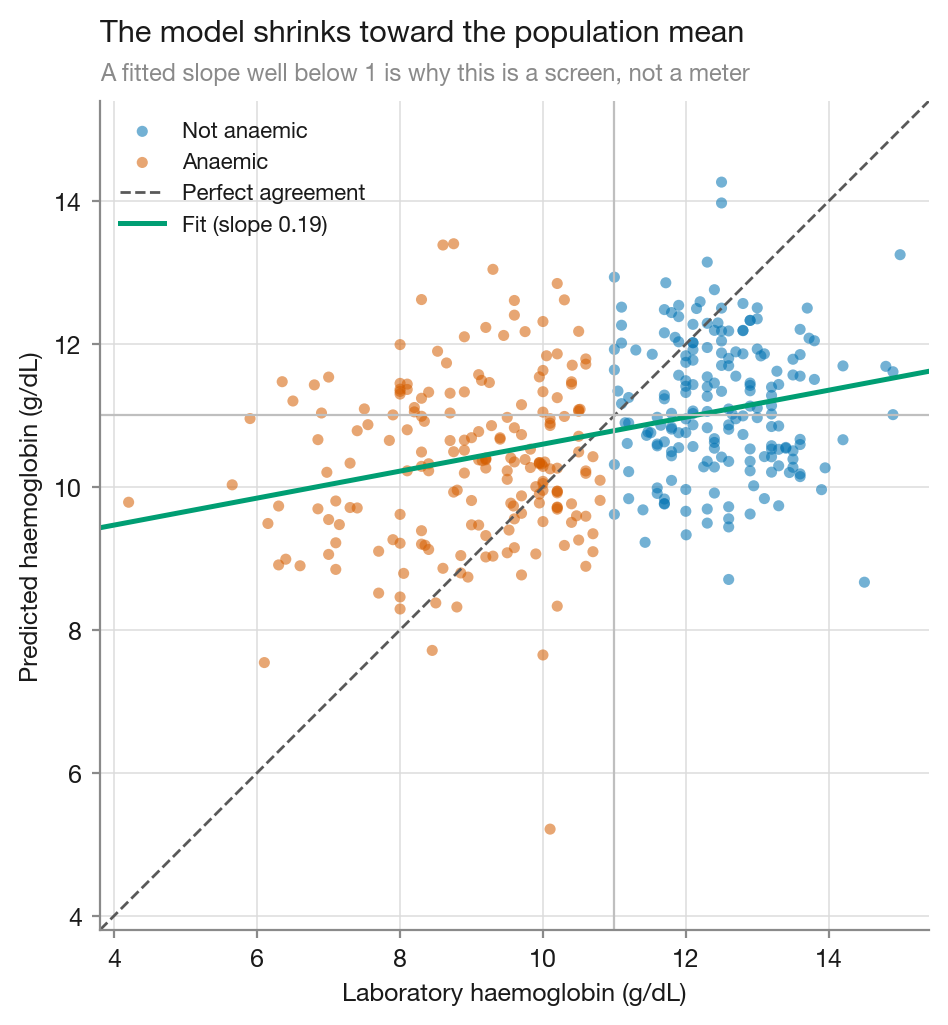
\includegraphics[width=0.60\textwidth]{../results/fig10_pred_vs_actual.png}
\caption{Predicted against laboratory haemoglobin. A least-squares fit through the predictions has
slope $0.19$, far below the identity line: a 1~\gdl{} change in true haemoglobin moves the
prediction by roughly a fifth of that. The model separates anaemic from non-anaemic children
while carrying little information about \emph{how} anaemic they are.}
\label{fig:pva}
\end{figure}

\begin{figure}[htbp]
\centering
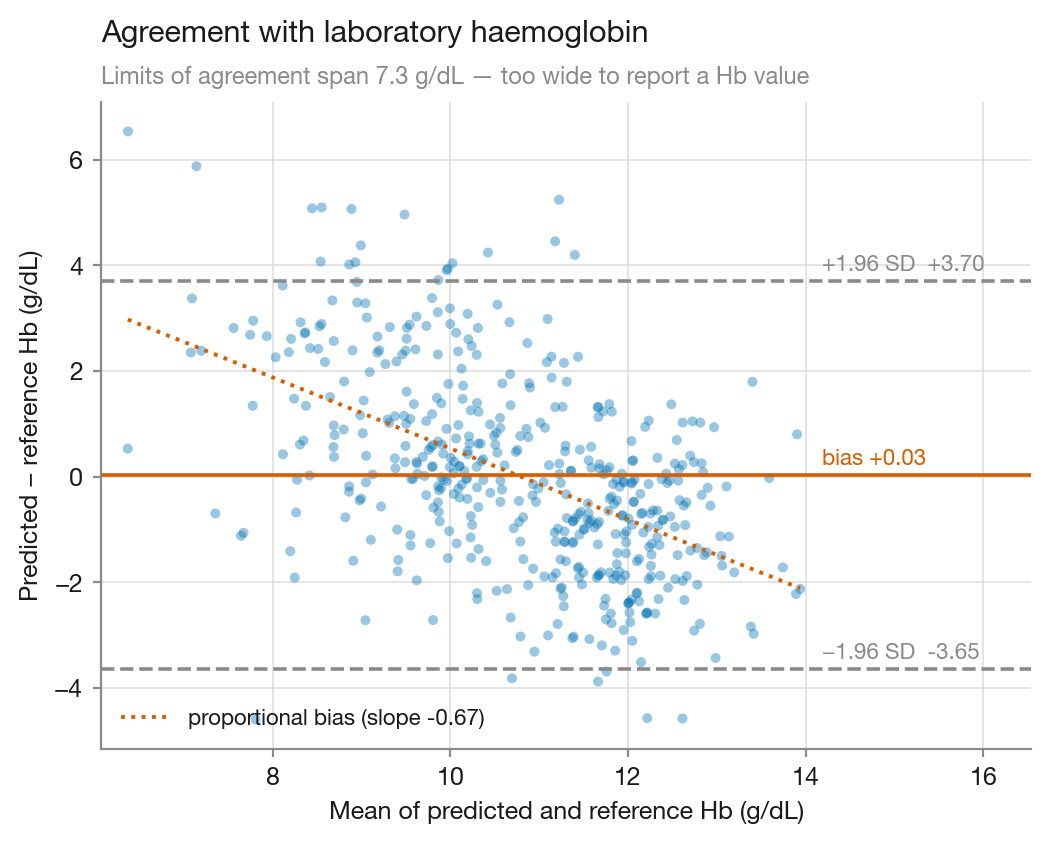
\includegraphics[width=0.68\textwidth]{../results/fig5_bland_altman.png}
\caption{Bland--Altman agreement. The limits span 7.8~\gdl{} and the proportional bias is
pronounced, establishing this as a triage screen rather than a measurement device.}
\label{fig:ba}
\end{figure}

\subsection{Is acting on the model better than the alternatives?}
\label{sec:dca}

Discrimination and calibration describe the model; neither says whether acting on it beats what a
clinic would otherwise do. Where the realistic comparators are ``refer every child'' and ``refer
none'', that comparison is what decides deployment. Decision curve analysis~\cite{vickers2006}
makes it directly, through net benefit

\begin{equation}
\mathrm{NB}(p_t) \;=\; \frac{\mathrm{TP}}{N} \;-\; \frac{\mathrm{FP}}{N}\cdot\frac{p_t}{1-p_t},
\end{equation}

where $p_t$ is the probability at which referral becomes worthwhile and the odds term prices one
missed case against the false referrals a clinic will tolerate for it. A model is worth using only
where its curve lies above both comparators.

Figure~\ref{fig:dca} shows the result, and it is a qualified one. \textbf{Below
$p_t \approx 0.26$ the model is worse than simply referring every child.} That is a direct
consequence of the 51\,\% prevalence in this cohort: when half the children are anaemic and
missing a case is judged far costlier than an unnecessary referral, no triage rule beats referring
everyone. Above that threshold the model does add benefit, and the margin widens as false
referrals become more costly.

The practical reading is that this model earns its place only where confirmatory testing is scarce
enough that indiscriminate referral is not an option. That is a narrower claim than \auroc{}
$0.706$ suggests on its own, and it is the claim the evidence supports. It is also a narrower
window than the same analysis indicated before the third deduplication pass, when the crossing
point stood at $p_t \approx 0.15$.

\begin{figure}[htbp]
\centering
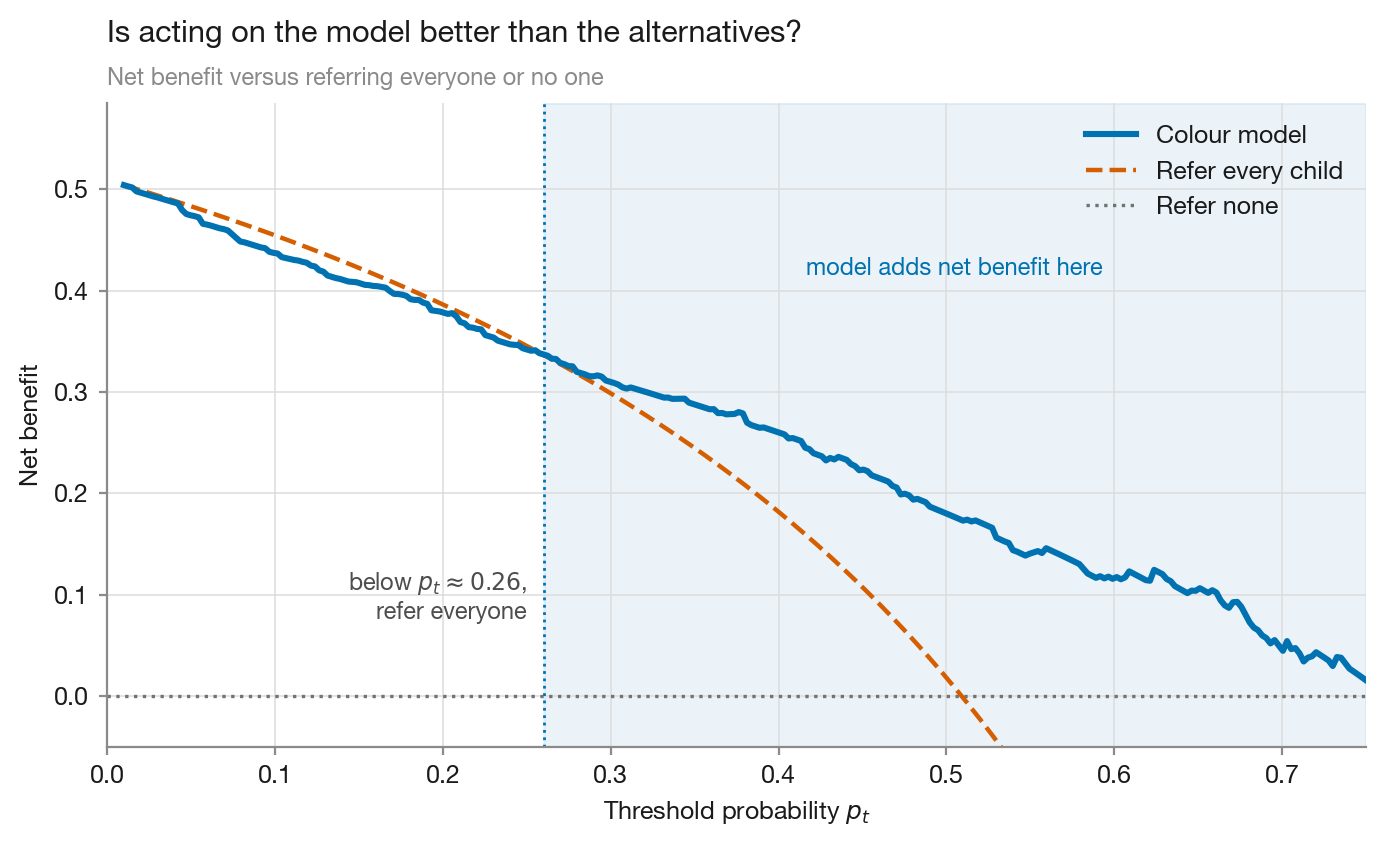
\includegraphics[width=0.82\textwidth]{../results/fig11_decision_curve.png}
\caption{Decision curve analysis. Net benefit of the colour model against the two comparators
available to a clinic. The model is not universally useful: below $p_t \approx 0.26$, referring every child is the better strategy, a consequence of the high
prevalence in this cohort. Its advantage appears once false referrals carry real cost.}
\label{fig:dca}
\end{figure}

\subsection{Cross-site generalisation}

Leave-one-site-out evaluation across nine evaluable hospitals gives a mean \auroc{} of
$0.722$ (range $0.606$--$0.875$); the tenth site contributes three photographs and cannot be
scored alone. The highest score, $0.875$ at SDA Hospital, rests on ten photographs at 80\,\%
prevalence and should be read as noise rather than performance. The informative observation is
that one of the two largest sites, Komfo Anokye Teaching Hospital ($n=68$), returns the lowest
score of all at $0.606$, while the other, Ahmadiyya Muslim Hospital ($n=68$), returns $0.747$.
Read the large sites rather than the mean: generalisation to an unseen hospital is nearer $0.7$
than the $0.722$ average, and the spread across sites is wide enough that a single-site pilot
would not establish much.

\begin{figure}[htbp]
\centering
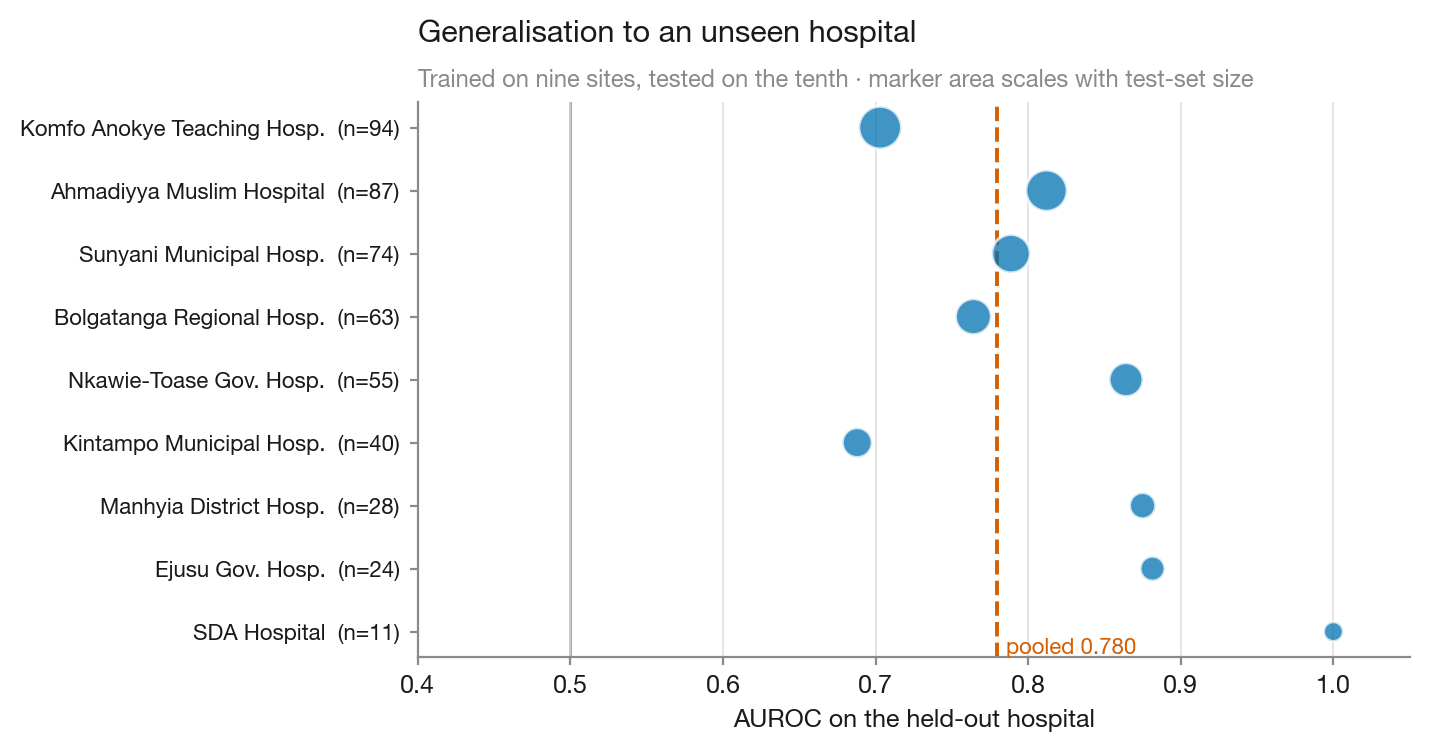
\includegraphics[width=0.72\textwidth]{../results/fig3_sites.png}
\caption{Leave-one-site-out performance. Marker area scales with test-set size; no interval is
drawn, but the smallest sites (SDA, $n=10$; Ejusu, $n=18$) are estimated from too few children to
support comparison, which is why we read the two largest sites instead.}
\label{fig:sites}
\end{figure}

\subsection{Which features carry the signal}

Permutation importance was measured out-of-fold (Figure~\ref{fig:imp}), because the model's
internal impurity importances are computed on training data and are biased toward continuous
features.
Four features share the lead within overlapping error bars: circular mean hue
($\Delta$\auroc{} $0.042$), mean saturation ($0.041$), the 10th percentile of the redness index
($0.041$) and the redness index itself ($0.040$), followed by mean red ($0.036$). Hue, saturation
and the pale tail of the redness distribution are the physiologically expected carriers of
pallor. Because these features are strongly correlated, a low score should be read as ``redundant
given the others'', not ``irrelevant''. Figure~\ref{fig:corr} shows this rather than assuming it:
mean absolute pairwise correlation across the twelve features is $0.52$, reaching $0.98$ between
mean green and CIELAB $L^*$. Two clusters are visible --- an RGB/lightness group and a
saturation-and-redness group --- and permutation importance divides credit within each. That is
why no single feature exceeds $0.05$ even though the set as a whole carries $+0.182$ \auroc{}
over demographics.

\begin{figure}[htbp]
\centering
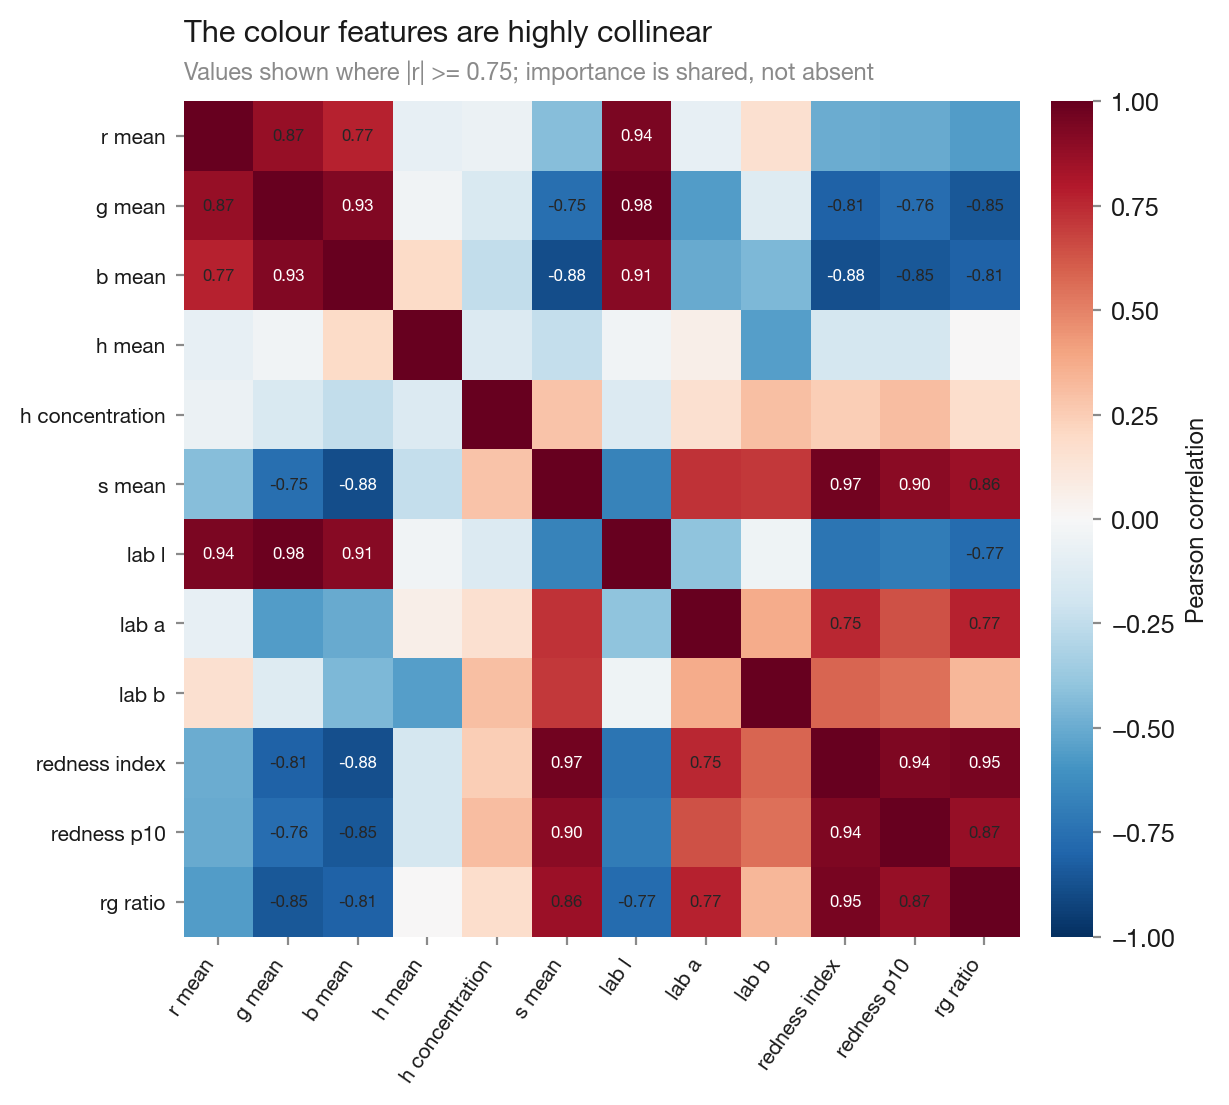
\includegraphics[width=0.70\textwidth]{../results/fig12_feature_correlation.png}
\caption{Pairwise correlation between the twelve colour features, printed where
$|r| \geq 0.75$. This collinearity is why a low permutation-importance score should be read as
redundancy given the rest of the set rather than absence of signal.}
\label{fig:corr}
\end{figure}

\begin{figure}[htbp]
\centering
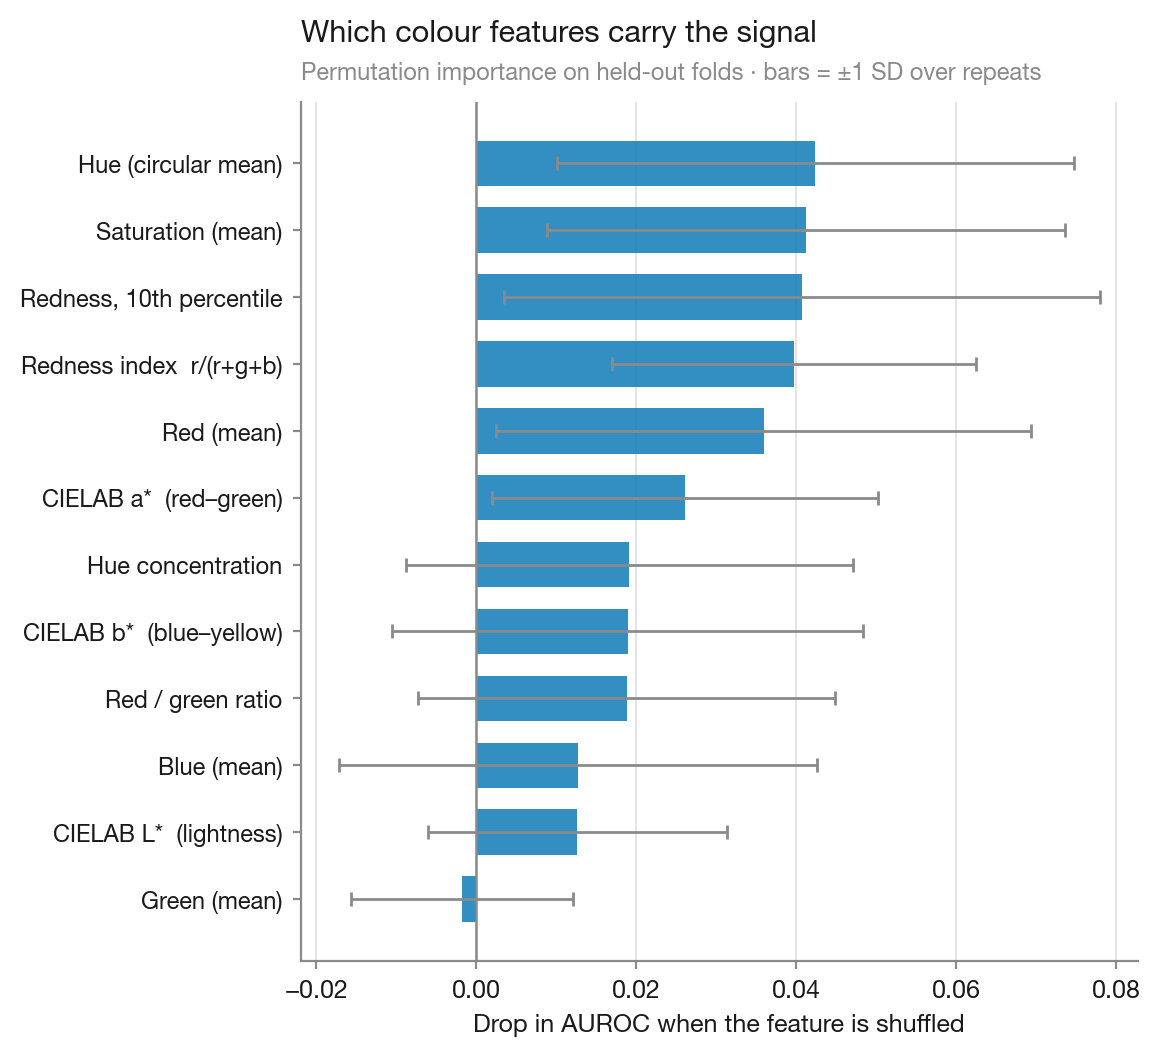
\includegraphics[width=0.68\textwidth]{../results/fig6_importance.png}
\caption{Out-of-fold permutation importance. Hue, saturation and the pale tail of the redness
distribution lead, within overlapping error bars. Correlated features share credit, so a low score
means redundant given the others rather than uninformative.}
\label{fig:imp}
\end{figure}

\subsection{Controls}
\label{sec:controls}

Table~\ref{tab:controls} lists checks designed to make the headline result fail if it were an
artefact. Three deserve comment.

The \emph{byte-hash singles} control keeps only files whose SHA-256 appears exactly once. It
scores $0.763$, above the headline --- and that is the expected direction, not a contradiction:
re-encoded and shifted copies have unique hashes, so they survive this filter, and the subset is
therefore not duplicate-free. We report it as a robustness check on the hash grain and no longer,
as we did previously, as a subset ``where no label conflict is possible''.

\emph{Nested cross-validation} now returns a \emph{lower} score than the fixed hyperparameters
($0.662$ against $0.706$). Tuning inside each fold at $n=383$ overfits the inner split; the
control's purpose --- showing the fixed settings were not selected for flattery --- is served, in
the more convincing direction.

The \emph{matched-$n$ control} separates the two things pass 3 does. Subsampling the
479-photograph set to 383 rows without removing any duplicates scores $0.744\pm0.021$, midway
between $0.780$ and $0.706$: the pass-3 drop is about half sample size and about half leakage.
This does not change the headline --- $0.706$ is what the model achieves on data that are actually
distinct, which is the number a deployment would face --- but it does bound how much of the fall
is attributable to contamination.

The \emph{alignment threshold sweep} is the least stable control. Between thresholds $1.0$ and $4.0$
the retained count falls from 397 to 376 while \auroc{} varies non-monotonically between $0.685$
and $0.728$: roughly $\pm0.02$ around the headline. The gap between merged and distinct pairs is real but narrower
than at pass 2, so we report the range rather than a single number, and we chose the threshold by
inspecting the borderline pairs by eye before seeing their effect on \auroc{}.

\begin{table}[htbp]
\centering
\caption{Adversarial and robustness controls.}
\label{tab:controls}
\footnotesize
\begin{tabular}{lll}
\toprule
Control & Result & Interpretation \\
\midrule
Label permutation (10 repeats)   & \auroc{} $0.529\pm0.032$ & chance; the harness does not leak \\
Seed stability (10 seeds)        & $0.702\pm0.006$          & not fold-assignment luck \\
Byte-hash singles only ($n=407$) & 0.763                    & higher, as expected: copies survive this filter \\
Nested-CV hyperparameter tuning  & $0.706 \to 0.662$        & fixed settings not cherry-picked \\
Re-encode threshold sweep (0.5--5.0) & 0.697--0.712         & insensitive to the pass-2 cutoff \\
Alignment threshold sweep (1.0--4.0) & 0.685--0.728, $n$ 397--376 & moderately sensitive; reported \\
Matched-$n$ control for pass 3 (25 draws) & $0.744\pm0.021$ & half the pass-3 drop is sample size \\
\bottomrule
\end{tabular}
\end{table}

\begin{figure}[htbp]
\centering
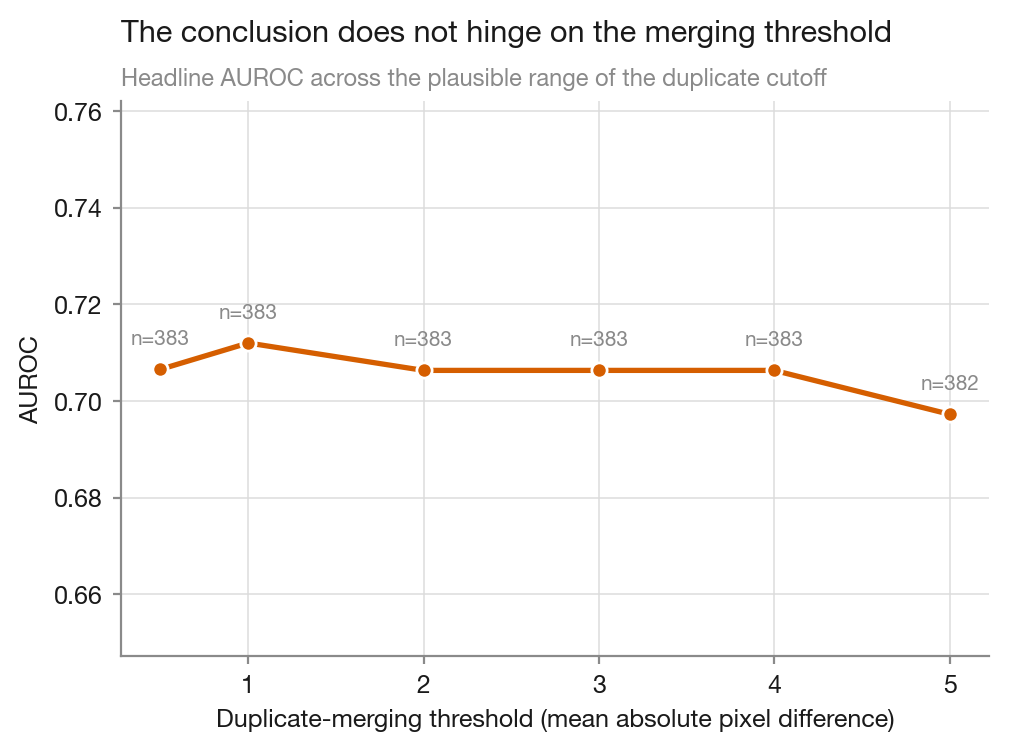
\includegraphics[width=0.66\textwidth]{../results/fig8_threshold.png}
\caption{Sensitivity of the headline result to the pass-2 re-encode detection threshold.
\auroc{} varies between 0.697 and 0.712 across the sweep, so the conclusion does not depend on
where this cutoff is placed.}
\label{fig:thr}
\end{figure}

\subsection{Would more data help?}

A learning curve over training-set size (Figure~\ref{fig:lc}) rises from \auroc{} $0.575$ at a
quarter of the data to
$0.704$ at full size and has not plateaued, though the ascent is not monotone --- the 70\,\%
point dips below the 55\,\% point, within the repeat-to-repeat spread the shaded band shows.
Performance here is therefore plausibly limited by sample size as well as by the dataset's
irreducible label noise --- and the third deduplication pass has made
the first constraint tighter, since the usable set is now 383 photographs rather than 479. A
larger, cleanly labelled dataset would plausibly exceed $0.706$.

\begin{figure}[htbp]
\centering
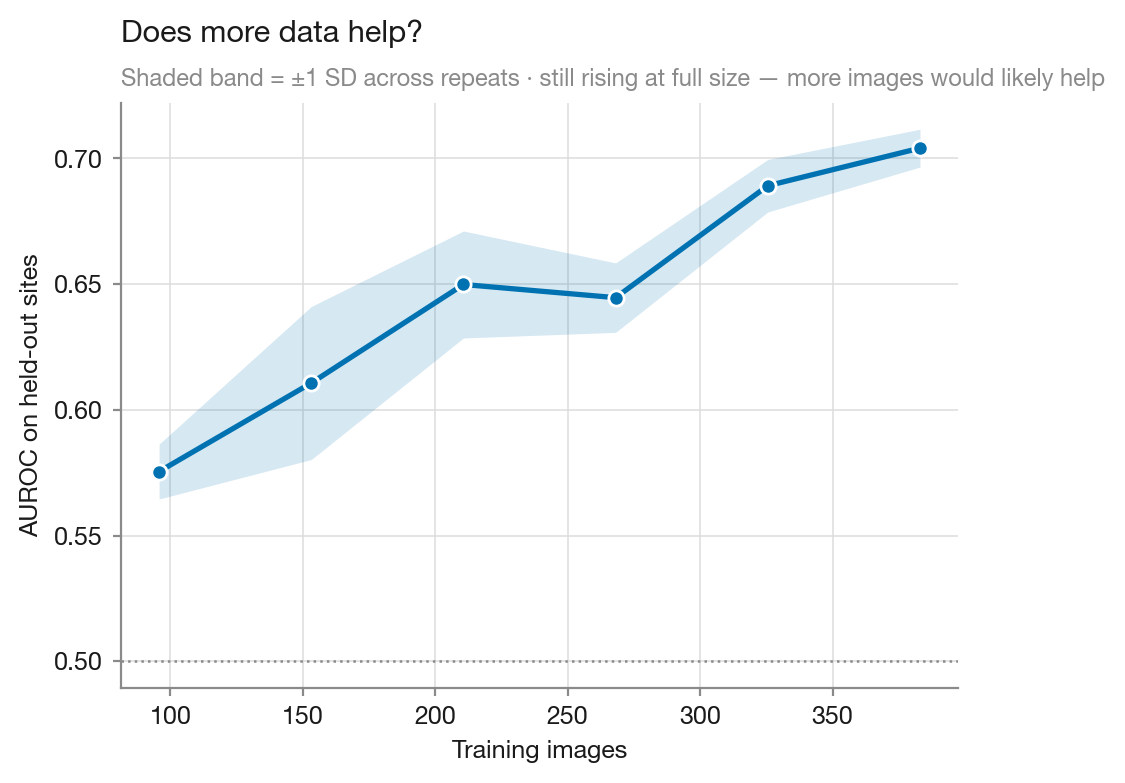
\includegraphics[width=0.66\textwidth]{../results/fig7_learning_curve.png}
\caption{Learning curve. The absence of a plateau indicates the benchmark is sample-limited.}
\label{fig:lc}
\end{figure}

\section{Discussion}

The gap between $0.883$ and $0.706$ is an artefact of dataset handling rather than a modelling
result. It matters because it is the kind of gap that separates a method reported as promising
from one reported as marginal, and because nothing about the naive protocol looks careless from
the inside --- a random split is the default, and duplicates are invisible unless specifically
sought.

Each form of duplication defeats the remedy for the previous one. The 19 re-encoded copies defeat a
practitioner who deduplicates by file hash. The 96 shifted copies defeat the obvious repair: they
survive pixel comparison too, because the hand-drawn mask moves with them, and 74 of the
photographs they conceal are attributed to more than one hospital, so they survive site-grouped
folds as well.
Two independent safeguards, each individually sound, leave the leak in place.

Half of the last step's cost is sample size rather than contamination; the
corrected number is lower both because the data are cleaner and because there are fewer of them,
and a benchmark of 383 photographs is small for the task.

An earlier version of this analysis applied passes 1 and 2, grouped folds by site, and reported
$0.780$ as the corrected figure; the residual leak was found only when we searched specifically for
copies whose masks disagreed. The general lesson we
draw is that dataset audits should be reported as a specific list of what was tested for, since
``deduplicated'' names a procedure rather than a property, and each procedure has a blind spot
that the next one exposes. We make no claim that a fourth form is absent from CP-AnemiC; we claim
only that these three are present and that the detector for each is public.

Our corrected baseline should be read as establishing a floor for interpretable colour
features, not a ceiling for the task. Learned representations may well exceed it. The
purpose of reporting it is that any such claim can now be measured against a number produced
under controls that are stated and reproducible.

Clinically, discrimination at \auroc{} $0.706$ remains of some
interest for triage where the alternative is no screening at all, but the margin has narrowed.
The Bland--Altman result forecloses use as a haemoglobin estimator; the operating point ---
70\,\% of healthy children referred at 90\,\% sensitivity --- would impose a confirmatory
testing burden that may exceed what a low-resource clinic can absorb; and the decision curve now
places the useful window above $p_t \approx 0.26$ rather than $0.15$. All three are more
decision-relevant than the \auroc{} that such studies typically headline, and all three moved
adversely when the evaluation set was corrected.

\section{Limitations}

\begin{itemize}
  \item \textbf{Label noise is irreducible.} At the final grain, 116 groups carry conflicting
        haemoglobin on the same photograph; median merging cannot recover the truth, and a
        performance ceiling is therefore built into the benchmark.
  \item \textbf{Deduplication is a floor, not a guarantee.} We detect three forms of
        duplication and cannot exclude a fourth. The alignment pass searches integer
        translations only: a copy that was rotated, rescaled or re-illuminated would evade it.
        The retained count varies between 376 and 397 photographs across defensible
        thresholds (Section~\ref{sec:controls}).
  \item \textbf{No colour calibration.} No colour card or white-balance reference was
        captured, so absolute RGB partly encodes illumination. Normalised ratios mitigate
        but do not eliminate this.
  \item \textbf{One country, one age band.} Children 6--59 months in Ghana. Nothing here
        supports use in adults, in pregnancy, or across different skin tones and camera
        pipelines.
  \item \textbf{Hand-drawn masks.} A deployed system would require automatic conjunctiva
        segmentation, whose error is not represented in any number reported here.
  \item \textbf{No true external validation.} Leave-one-site-out varies camera, operator and
        prevalence, but not country or protocol --- and site attribution is itself unreliable
        here, since 125 duplicate groups span more than one hospital. Validation on an
        independent dataset is the obvious next step.
  \item \textbf{Not a clinical device.} No regulatory, ethical or safety assessment has been
        performed. This is a software study on a public dataset.
\end{itemize}

\section{Conclusion}

CP-AnemiC's 710 records resolve to 383 distinct photographs. The duplication takes three forms
--- byte-identical files, re-encoded copies, and shifted or re-cropped copies that survive both
content hashing and aligned pixel comparison --- and inflates \auroc{} by approximately $0.18$
under a random split. Because 125 duplicate groups are attributed to more than one hospital, the
duplication also defeats site-grouped cross-validation. We recommend that future work on this
benchmark deduplicate under small translations, group folds by site, and state which forms of
duplication were tested for.

Under those controls, twelve interpretable colour features achieve \auroc{} $0.706$
(95\,\% CI $0.653$--$0.757$) for WHO childhood anaemia, with the image contributing $+0.182$
over demographics alone. The resulting model is a plausible triage screen and is not a
haemoglobin meter: limits of agreement span $7.8$~\gdl{} and specificity falls to $0.303$ at
90\,\% sensitivity. Reporting these quantities alongside \auroc{} is, we suggest, the minimum
needed to judge whether such a method could be deployed.

\section*{Reproducibility}

The complete analysis runs in approximately nine minutes on a laptop --- dominated by the
alignment pass; its pairwise distances are cached, and subsequent runs take about 90~seconds:

\begin{quote}\ttfamily\small
pip install -r requirements.txt\\
\# download CP-AnemiC into data/cp-anemic/\\
python3 scripts/run\_full\_analysis.py\\
python3 -m pytest tests/ -q
\end{quote}

Every number and figure in this paper is regenerated by that script. The accompanying test
suite (62 tests) is organised by failure mode --- split integrity, feature correctness,
numerical robustness, determinism, statistical machinery, and adversarial nulls --- on the
principle that the dangerous failure in this setting is not a crash but a plausible wrong
number.

\section*{Declarations}

\noindent\textbf{Use of generative AI.} Manuscript text and analysis code were drafted with
generative AI assistance (Anthropic Claude) under the author's direction. The author has verified
the manuscript and takes full responsibility for its content.

\section*{Data availability}

CP-AnemiC is publicly available from Mendeley Data
(\href{https://data.mendeley.com/datasets/m53vz6b7fx/1}{\texttt{m53vz6b7fx}})
\cite{asare2023cpanemic} and is used under its published licence. No patient-identifiable
data is redistributed. Derived colour statistics only are stored in the accompanying
repository.

\section*{Conflicts of interest}

None declared.

\begin{thebibliography}{9}

\bibitem{asare2023cpanemic}
J.~W. Asare, P.~Appiahene, and E.~T. Donkoh,
\newblock ``CP-AnemiC: A conjunctival pallor dataset and benchmark for anemia detection in
children,''
\newblock \emph{Mendeley Data}, \texttt{m53vz6b7fx}, 2023.

\bibitem{stevens2022}
G.~A. Stevens, C.~J. Paciorek, M.~C. Flores-Urrutia, et al.,
\newblock ``National, regional, and global estimates of anaemia by severity in women and children
for 2000--19: a pooled analysis of population-representative data,''
\newblock \emph{The Lancet Global Health}, vol.~10, no.~5, pp.~e627--e639, 2022.

\bibitem{who2011}
World Health Organization,
\newblock ``Haemoglobin concentrations for the diagnosis of anaemia and assessment of
severity,''
\newblock \emph{Vitamin and Mineral Nutrition Information System}, WHO/NMH/NHD/MNM/11.1,
Geneva, 2011.

\bibitem{vickers2006}
A.~J. Vickers and E.~B. Elkin,
\newblock ``Decision curve analysis: a novel method for evaluating prediction models,''
\newblock \emph{Medical Decision Making}, vol.~26, no.~6, pp.~565--574, 2006.

\bibitem{delong1988}
E.~R. DeLong, D.~M. DeLong, and D.~L. Clarke-Pearson,
\newblock ``Comparing the areas under two or more correlated receiver operating
characteristic curves: a nonparametric approach,''
\newblock \emph{Biometrics}, vol.~44, no.~3, pp.~837--845, 1988.

\bibitem{blandaltman1986}
J.~M. Bland and D.~G. Altman,
\newblock ``Statistical methods for assessing agreement between two methods of clinical
measurement,''
\newblock \emph{The Lancet}, vol.~327, no.~8476, pp.~307--310, 1986.

\end{thebibliography}

\end{document}
